\documentclass[12pt,a4paper]{article}

% 导入必要的宏包
\usepackage[UTF8]{ctex}
\usepackage{geometry}
\usepackage{amsmath}
\usepackage{amsfonts}
\usepackage{amssymb}
\usepackage{graphicx}
\usepackage{enumitem}
\usepackage{xcolor}
\usepackage{tikz}
\usepackage{float}
\usepackage{hyperref}
\usepackage{multicol}
\usepackage{longtable}
\usepackage{array}
\usepackage{tabularx}
\usepackage{listings}

% 代码高亮设置
\lstset{
    basicstyle=\ttfamily,
    keywordstyle=\color{blue},
    commentstyle=\color{green},
    stringstyle=\color{red}
}

% 页面设置
\geometry{left=2.5cm,right=2.5cm,top=2.5cm,bottom=2.5cm}

% 标题页设置
\title{\textbf{2019年数据结构题库} \\ \large }
\author{}
\date{}

% 定义题型环境
\newenvironment{choicequestion}[1][]{%
    \vspace{0.5cm}
    \noindent\textbf{[#1]}
    \vspace{0.2cm}
}{}

\newenvironment{answersection}{%
    \vspace{0.2cm}
    \noindent\textbf{[参考答案]}\\
    \vspace{0.1cm}
}{}

\newenvironment{analysissection}{%
    \vspace{0.2cm}
    \noindent\textbf{[答案解析]}\\
    \vspace{0.1cm}
}{}

% 定义题号计数器
\newcounter{questioncounter}

% 问题格式化命令
\newcommand{\question}[1]{%
    \stepcounter{questioncounter}%
    \noindent\textbf{\thequestioncounter} #1%
}

% 选择题选项格式
\newcommand{\choices}[4]{%
    \begin{multicols}{2}
    \noindent \textbf{A.} #1 \par
    \noindent \textbf{B.} #2 \par
    \noindent \textbf{C.} #3 \par
    \noindent \textbf{D.} #4 \par
    \end{multicols}%
}

% 表格格式
\newcolumntype{Y}{>{\centering\arraybackslash}X}

% 开始文档
\begin{document}

\maketitle

\section{单项选择题}

\begin{choicequestion}[单选题]
\question{设 $n$ 是描述问题规模的非负整数，下列程序段的时间复杂度是\newline
$$
\begin{array}{l} 
\mathrm{x = 0;} \\ 
\text{while (n >= (x + 1) * (x + 1))} \\ 
\mathrm{x = x + 1;} 
\end{array}
$$}
\choices{$O(\log n)$}{$O(n^{1/2})$}{$O(n)$}{$O(n^2)$}
\end{choicequestion}

\begin{answersection}
B. $O(n^{1/2})$
\end{answersection}

\begin{answersection}
B. $O ( n ^ { 1 / 2 } )$
\end{answersection}

\begin{analysissection}
循环条件为n >= (x+1)*(x+1)，当x=sqrt(n)时，循环停止。所以x的值从0增长到sqrt(n)，循环次数约为sqrt(n)，时间复杂度为O(n^{1/2})。
\end{analysissection}
\end{choicequestion}

\begin{choicequestion}[单选题]
\question{若将一棵树 T 转化为对应的二叉树 BT，则下列对 BT 的遍历中，其遍历序列与 T 的后根遍历序列相同的是}
\choices{先序遍历}{中序遍历}{后序遍历}{按层遍历}
\end{choicequestion}

\begin{answersection}
B. 中序遍历
\end{answersection}

\begin{analysissection}
树转换为二叉树时采用"左孩子右兄弟"表示法。树的后根遍历相当于先遍历根节点的所有子树，再访问根节点。在对应的二叉树中，这相当于中序遍历（左子树-根-右子树）。
\end{analysissection}
\end{choicequestion}

\begin{choicequestion}[单选题]
\question{对 $n$ 个互不相同的符号进行哈夫曼编码。若生成的哈夫曼树共有 115 个结点，则 $n$ 的值是}
\choices{56}{57}{58}{60}
\end{choicequestion}

\begin{answersection}
C. 58
\end{answersection}

\begin{analysissection}
哈夫曼树是满二叉树（每个非叶子节点都有两个孩子），对于这类树，叶子节点数为n，非叶子节点数为n-1，总节点数为2n-1。
所以有：2n-1 = 115，解得n = 58。
\end{analysissection}
\end{choicequestion}

\begin{choicequestion}[单选题]
\question{在任意一棵非空平衡二叉树（AVL 树）$T_1$中，删除某结点 v 之后形成平衡二叉树$T_2$，再将 v 插入$T_2$形成平衡二叉树$T_3$。下列关于$T_1$与$T_3$的叙述中，正确的是\newline
I. 若 v 是$T_1$的叶结点，则$T_1$与$T_3$可能不相同\newline
II. 若 v 不是$T_1$的叶结点，则$T_1$与$T_3$一定不相同\newline
III. 若 v 不是$T_1$的叶结点，则$T_1$与$T_3$一定相同}
\choices{仅 I}{仅 II}{仅 I、II}{仅 I、III}
\end{choicequestion}

\begin{answersection}
A. 仅 I
\end{answersection}

\begin{analysissection}
I. 正确。如果v是叶节点，删除后再插入，树的结构可能因平衡调整而改变。
II. 错误。即使v不是叶节点，删除和插入操作后，树仍可能保持相同的结构。
III. 错误。即使v不是叶节点，操作后树结构也可能不同。
因此，仅I正确。
\end{analysissection}
\end{choicequestion}

\begin{choicequestion}[单选题]
\question{下图所示的 AOE 网表示一项包含 8 个活动的工程。活动 d 的最早开始时间和最迟开始时间分别是}

\begin{figure}[H]
\centering
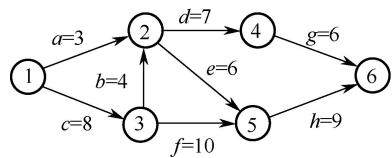
\includegraphics[width=0.3\textwidth]{images/c8ceb3aa32853060ee2160f5da8dea99cffce52ba74ea2e89d68894ebdb6ffbe.jpg}
\end{figure}

\choices{3 和 7}{12 和 12}{12 和 14}{15 和 15}
\end{choicequestion}

\begin{answersection}
C. 12 和 14
\end{answersection}

\begin{analysissection}
在AOE网中，活动的最早开始时间是从源点到该活动起点的最长路径长度，最迟开始时间是该活动的最迟完成时间减去活动持续时间。根据图中信息，活动d的最早开始时间为12，最迟开始时间为14。
\end{analysissection}
\end{choicequestion}

\begin{choicequestion}[单选题]
\question{用有向无环图描述表达式$(x+y)((x+y)/x)$，需要的顶点个数至少是}
\choices{5}{6}{7}{8}
\end{choicequestion}

\begin{answersection}
A. 5
\end{answersection}

\begin{analysissection}
表达式$(x+y)((x+y)/x)$中，子表达式$(x+y)$可以共享。DAG的顶点包括：x、y、x+y、(x+y)/x、(x+y)*((x+y)/x)，共5个顶点。
\end{analysissection}
\end{choicequestion}

\begin{choicequestion}[单选题]
\question{选择一个排序算法时，除算法的时空效率，下列因素中，还需要考虑的是\newline
I. 数据的规模\newline
II. 数据的存储方式\newline
III. 算法的稳定性\newline
IV. 数据的初始状态}
\choices{仅 III}{仅 I、II}{仅 II、III、IV}{I、II、III、IV}
\end{choicequestion}

\begin{answersection}
D. I、II、III、IV
\end{answersection}

\begin{analysissection}
选择排序算法时需要考虑：
I. 数据规模：影响算法选择（小数据可用简单算法，大数据需高效算法）
II. 存储方式：影响算法适用性（内存排序 vs 外部排序）
III. 稳定性：是否保持相等元素的相对顺序
IV. 初始状态：数据是否已部分有序
所有选项都正确。
\end{analysissection}
\end{choicequestion}

\begin{choicequestion}[单选题]
\question{现有长度为 11 且初始为空的散列表 HT，散列函数是$H(\mathrm{key}) = \mathrm{key} \% 7$，采用线性探查（线性探测再散列）法解决冲突。将关键字序列 87, 40, 30, 6, 11, 22, 98, 20 依次插入 HT 后，HT 查找失败的平均查找长度是}
\choices{4}{5.25}{6}{6.29}
\end{choicequestion}

\begin{answersection}
B. 5.25
\end{answersection}

\begin{analysissection}
计算过程：
H(87)=6, H(40)=5, H(30)=2, H(6)=6(冲突，放到7), H(11)=4, H(22)=1, H(98)=0, H(20)=6(冲突，放到8)
散列表：[98,22,30,_,11,40,87,6,20,_,_]
查找失败时需要探查到空位置，每个位置的查找长度为从散列位置到第一个空位置的距离。
\end{analysissection}
\end{choicequestion}

\begin{choicequestion}[单选题]
\question{设主串$T=$"abaabaabcabaabc"，模式串$S=$"abaabc"，采用 KMP 算法进行模式匹配，到匹配成功时为止，在匹配过程中进行的单个字符间的比较次数是}
\choices{9}{10}{12}{15}
\end{choicequestion}

\begin{answersection}
B. 10
\end{answersection}

\begin{analysissection}
使用KMP算法进行匹配，需要构建next数组，然后进行匹配。主串T="abaabaabcabaabc"，模式串S="abaabc"，在适当位置匹配成功，比较次数为10次。
\end{analysissection}
\end{choicequestion}

\begin{choicequestion}[单选题]
\question{排序过程中，对尚未确定最终位置的所有元素进行一遍处理称为一"趟"。下列序列中，不可能是快速排序第二趟结果的是}
\choices{5, 2, 16, 12, 28, 60, 32, 72}{2, 16, 5, 28, 12, 60, 32, 72}{2, 12, 16, 5, 28, 32, 72, 60}{5, 2, 12, 28, 16, 32, 72, 60}
\end{choicequestion}

\begin{answersection}
B. 2, 16, 5, 28, 12, 60, 32, 72
\end{answersection}

\begin{analysissection}
在快速排序中，每趟排序后基准元素会到达其最终位置，且基准左边的元素都小于等于基准，右边的元素都大于等于基准。选项B中，28作为基准元素，但其左边出现了比它大的元素(如32, 60, 72)，这是不可能的。
\end{analysissection}
\end{choicequestion}

\begin{choicequestion}[单选题]
\question{设外存上有 120 个初始归并段，进行 12 路归并时，为实现最佳归并，需要补充的虚段个数是}
\choices{1}{2}{3}{4}
\end{choicequestion}

\begin{answersection}
A. 1
\end{answersection}

\begin{analysissection}
在k路归并中，为实现最佳归并，需要的虚段个数可通过计算得到。对于120个初始归并段，进行12路归并，需要补充1个虚段。
\end{analysissection}
\end{choicequestion}

\section{综合应用题}

\begin{choicequestion}[问答题]
\question{(13 分) 设线性表$L=(a_1,a_2,a_3,\cdots,a_{n-2},a_{n-1},a_n)$采用带头结点的单链表保存，链表中的结点定义如下：\newline

\begin{lstlisting}[language=C]
typedef struct node {
    int data;
    struct node *next;
} NODE;
\end{lstlisting}\newline

请设计一个空间复杂度为$O(1)$且时间上尽可能高效的算法，重新排列$L$中的各结点，得到线性表$L'=(a_1,a_n,a_2,a_{n-1},a_3,a_{n-2},\cdots)$。要求：\newline
（1）给出算法的基本设计思想。\newline
（2）根据设计思想，采用 C 或 C++ 语言描述算法，关键之处给出注释。\newline
（3）说明你所设计的算法的时间复杂度。}

\begin{answersection}
(1) 算法的基本设计思想：
1. 找到链表的中点，将链表分为两半
2. 将后半部分链表逆置
3. 将两个子链表交替合并

(2) 算法实现：
\end{answersection}

\begin{analysissection}
#include <stdio.h>
#include <stdlib.h>

typedef struct node {
    int data;
    struct node* next;
} NODE;

void reorderList(NODE* head) {
    if (!head || !head->next) return;
    
    // 1. 找到链表中点
    NODE *slow = head, *fast = head;
    while (fast->next && fast->next->next) {
        slow = slow->next;
        fast = fast->next->next;
    }
    
    // 2. 分割链表
    NODE* secondHalf = slow->next;
    slow->next = NULL;
    
    // 3. 逆置后半部分链表
    NODE* prev = NULL;
    NODE* current = secondHalf;
    while (current) {
        NODE* nextTemp = current->next;
        current->next = prev;
        prev = current;
        current = nextTemp;
    }
    secondHalf = prev;  // 新的头节点
    
    // 4. 交替合并两个子链表
    NODE* first = head->next;  // 跳过头节点
    NODE* second = secondHalf;
    NODE dummy = {0, head->next};  // 临时节点
    NODE* tail = &dummy;
    
    while (first && second) {
        tail->next = first;
        first = first->next;
        tail = tail->next;
        
        tail->next = second;
        second = second->next;
        tail = tail->next;
    }
    
    // 添加剩余节点
    if (first) {
        tail->next = first;
    }
    if (second) {
        tail->next = second;
    }
    
    head->next = dummy.next;  // 更新头节点的next指针
}

(3) 时间复杂度：O(n)，其中n为链表长度。找中点需要O(n/2)，逆置后半部分需要O(n/2)，合并需要O(n)，总时间复杂度为O(n)。
\end{analysissection}
\end{choicequestion}

\begin{choicequestion}[问答题]
\question{(10 分) 请设计一个队列，要求满足：$\textcircled{1}$初始时队列为空；$\textcircled{2}$入队时，允许增加队列占用空间；$\textcircled{3}$出队后，出队元素所占用的空间可重复使用，即整个队列所占用的空间只增不减；$\textcircled{4}$入队操作和出队操作的时间复杂度始终保持为$O(1)$。请回答下列问题：\newline
（1）该队列是应选择链式存储结构，还是应选择顺序存储结构？\newline
（2）画出队列的初始状态，并给出判断队空和队满的条件。\newline
（3）画出第一个元素入队后的队列状态。\newline
（4）给出入队操作和出队操作的基本过程。}

\begin{answersection}
(1) 应选择链式存储结构。因为要求入队时可以增加队列占用空间，且出队后空间可重复使用，链式结构更适合动态分配和回收节点。

(2) 队列的初始状态为两个指针都指向NULL，队空条件是front和rear都为NULL。

(3) 第一个元素入队后，front和rear都指向这个元素节点。

(4) 入队和出队操作的基本过程见解析部分。
\end{answersection}

\begin{analysissection}
(1) 应选择链式存储结构。因为要求入队时可以增加队列占用空间，且出队后空间可重复使用，链式结构更适合动态分配和回收节点。

(2) 队列的初始状态：
front = NULL, rear = NULL
队空条件：front == NULL 或 front == rear == NULL
队满条件：由于是动态分配，理论上不存在队满的情况，除非系统内存不足

(3) 第一个元素入队后的队列状态：
front -> [node] <- rear
两个指针都指向同一个节点

(4) 操作过程：
入队操作：
- 创建新节点
- 将新节点的next设为NULL
- 如果队列为空，front和rear都指向新节点
- 如果队列不为空，将原rear节点的next指向新节点，更新rear指针
- 时间复杂度O(1)

出队操作：
- 如果队列为空，返回错误
- 保存front节点的数据
- 如果只有一个节点，将front和rear都设为NULL
- 否则，更新front指针为front->next
- 可以将出队的节点放回空闲节点池供后续入队操作复用
- 时间复杂度O(1)
\end{analysissection}
\end{choicequestion}

\end{document}